\documentclass[aps,prd,nofootinbib,twocolumn,10pt]{revtex4-2}

\usepackage{amssymb,amsmath,hyperref}
\hypersetup{
	colorlinks=true,
	linktoc=page,
	citecolor=blue,
	linkcolor=blue,
	urlcolor=blue} 
\urlstyle{same}

\usepackage{natbib}

\usepackage{tikz}
\usetikzlibrary{arrows.meta}

\newcommand{\NN}{\mathcal{N}}
\newcommand{\OO}{\mathcal{O}}
\newcommand{\Aa}{\mathcal{A}}
\newcommand{\Tr}{\mathrm{Tr}}

\newcommand{\agl}[2]{\langle#1\, #2 \rangle}
\newcommand{\sqr}[2]{\lbrack #1\, #2 \rbrack}
\newcommand{\tlambda}{\widetilde{\lambda}}

\usepackage[colorinlistoftodos]{todonotes}
\setuptodonotes{color=cyan}
\presetkeys{todonotes}{inline}{}

\begin{document}

%%% --- Frontmatter --- %%%

\title{Generic EFT Operator Basis from 4D Spinor Helicity Formalism}	
\author{Stefano De Angelis}
\email{s.deangelis@qmul.ac.uk}
\affiliation{Centre for Theoretical Physics, School of Physics and Astronomy, Queen Mary University of London, Mile End Road, London E1 4NS, United Kingdom}
\date{\today} 
\begin{abstract}
     Something
\end{abstract}
	
	
% \maketitle
	
% \tableofcontents

% \listoftodos

% \section{Introduction}

% \section{Operators and Minimal Amplitudes}

% \todo{three-points are special, we do only four points - no special kinematics involved}

% Each effective interaction will be identified by its {\it minimal} amplitude, {\it i.e.} the amplitude at leading order which does not vanish in free theory (if we switch off all the other interactions). This has to be a contact term, {\it i.e.} there are no intermediate modes propagating.

% As a first step in the classification procedure, we fix the mass-dimension $\left[\mathcal{O}\right]$ of the marginal operators for which we want to find a complete basis. From the minimal amplitudes we strip off the coupling of the effective interaction, which is related to the dimension of the corresponding marginal operator by
% \begin{equation}
%     \left[g_{\mathcal{O}}\right] = 4-\left[\mathcal{O}\right]\ .
% \end{equation}
% What we are looking for are the kinematic structures which have mass dimension
% \begin{equation}
% \label{eq::dimcontact}
%     \left[\mathcal{O}\right]-n\geq 0\ ,
% \end{equation}
% where $n$ is the number of external legs in the corresponding minimal amplitude. Equation \eqref{eq::dimcontact} provides a constraint on $n$ which can be further refined by taking into account which types of particles are found in the amplitudes. In fact, in order to get helicity weights right, each vector in the minimal amplitude will contribute at least with two spinor variables and each fermion at least with one. This leads to the stronger constraint. This condition is not only necessary but also sufficient for having local interactions.
% \begin{equation}
% \label{eq::particleconstraint}
%  \left[\mathcal{O}\right] - n \geq \frac{1}{2} \cdot \left( 2\, n_g + n_f \right) \, \hspace{0.2em} \implies \hspace{0.2em} 2 n_g + \frac{3}{2} n_f + n_s \leq \left[\mathcal{O}\right]\ ,
% \end{equation}
% where $n_g$, $n_f$ and $n_s$ are respectively the number of vectors, fermions and scalars and clearly $n=n_g+n_f+n_s$.
% Next, we need to take into account the constraints coming from the condition that our kinematic structures must be ${\rm SL}(2,\mathbb{C})$ invariant. This requires to further distinguish between helicities of the different particles, and to find all the $(n_{g^-},n_{g^+},n_{f^-},n_{f^+},n_s)$. The superscript of the subscript specify the helicity of the particles: $n_g = n_{g^-}+n_{g^+}$ and  $n_f = n_{f^-}+n_{f^+}$. compatible with the constraint \eqref{eq::particleconstraint}.
% Once $n_g$, $n_f$ and $n_s$ are fixed, we take into account that every state can contribute to the kinematic structures with powers of its momentum, which correspond to derivates in the operator language. The total number of momenta $n_\partial$ is fixed by saturating the mass dimension constraint to
% \begin{equation}
%     n_\partial = \left[ \mathcal{O}\right] - 2 n_g - \frac{3}{2}n_f - n_s \> .
% \end{equation}

\section{The massless basis}

% In this section, we am going to present the graph-based method to find a basis of polynomial kinematic structures in a generic massless theory in four dimensions which are Poincaré invariant.
% \todo{explain Poicaré invariance}

\subsection{Kinematic structures from spinor helicity variables}
\label{sec:kinematics}

A simple way of finding all the possible Lorentz-invariant structures in four-dimensions is to identify them with an oriented graph with two kind of edges, where each vertex is associated to a particle, and the edges correspond to angle (red) or square (blue) ${\rm SL}(2,\mathbb{C})$ invariants, as shown in Figure~\ref{fig:2graphexample}. The orientation of the edges then keeps track of the ordering of particles in the spinor brackets and thus provides potential minus signs.

\begin{figure}[t]
	    \begin{center}
		    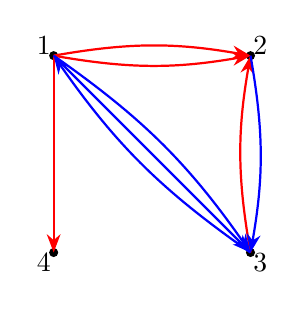
\begin{tikzpicture}[scale=2.5,>=Stealth]
		    
			    \node at (-0.05,-0.05) {$4$};
			    \node at (-0.05,1.05) {$1$};
			    \node at (1.05,1.05) {$2$};
			    \node at (1.05,-0.05) {$3$};
			    
			    \draw [fill] (0,0) circle [radius = 0.02];
			    \draw [fill] (1,0) circle [radius = 0.02];
			    \draw [fill] (0,1) circle [radius = 0.02];
			    \draw [fill] (1,1) circle [radius = 0.02];
			    
			    \draw [<-,thick,red](0,0) -- (0,1);
			    
			    \draw [->,thick,red](0,1) to [out=-10,in=-170] (1,1);
			    \draw [->,thick,red](0,1) to [out=10,in=-190] (1,1);
			    
			    \draw [<-,thick,red](1,1) to [out=-100,in=100] (1,0);
			    \draw [->,thick,blue](1,1) to [out=-80,in=80] (1,0);
			    
			    \draw [->,thick,blue](0,1) -- (1,0);
			    \draw [<-,thick,blue](0,1) to [out=-55,in=145] (1,0);
			    \draw [->,thick,blue](0,1) to [out=-35,in=125] (1,0);
	
		    \end{tikzpicture}
            \hspace{1cm}
	        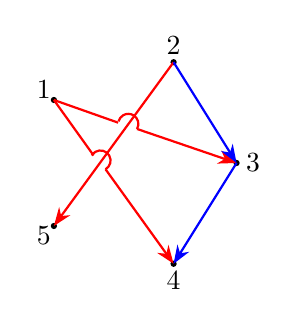
\begin{tikzpicture}[scale=1.6,>=Stealth]
	            
	            \node at (-0.08,-0.08) {$5$};
			    \node at (-0.08,1.08) {$1$};
			    \node at (0.95,1.43) {$2$};
			    \node at (1.58,0.5) {$3$};
			    \node at (0.95,-0.43) {$4$};
			    
			    \draw [fill] (0,0) circle [radius = 0.02];
			    \draw [fill] (0,1) circle [radius = 0.02];
			    \draw [fill] (0.95,1.3) circle [radius = 0.02];
			    \draw [fill] (1.45,0.5) circle [radius = 0.02];
			    \draw [fill] (0.95,-0.3) circle [radius = 0.02];
			    
			    %\draw [->,thick,red](0,1) -- (1.45,0.5);
			    %\draw [->,thick,red](0,1) -- (0.95,-0.3);
			    \draw [->,thick,red](0.95,1.3) -- (0,0);
			    
			    \draw [->,thick,red](0.41,0.45) -- (0.95,-0.3);
			    \draw [thick,red](0,1) -- (0.315,0.56);
			    \draw [thick,red] (0.41,0.45) arc (-60:150:0.08);
			    %\draw [fill] (0.315,0.56) circle [radius = 0.02];
			    %\draw [fill] (0.41,0.45) circle [radius = 0.02];
			    %\draw [fill] (0.66,0.77) circle [radius = 0.02];
			    %\draw [fill] (0.51,0.82) circle [radius = 0.02];
			    \draw [->,thick,red](0.66,0.77) -- (1.45,0.5);
			    \draw [thick,red](0,1) -- (0.51,0.82);
			    \draw [thick,red] (0.66,0.77) arc (-30:165:0.08);
			    
			    \draw [->,thick,blue](0.95,1.3) -- (1.45,0.5);
			    \draw [->,thick,blue](1.45,0.5) -- (0.95,-0.3);
	            
	        \end{tikzpicture}
	    \end{center}
    \caption{The graph associate to the kinematic structures $\textcolor{red}{\agl{1}{2}^2 \agl{1}{4} \agl{3}{2}} \textcolor{blue}{\sqr{2}{3}\sqr{1}{3}^2 \sqr{3}{1}}$ and $\textcolor{red}{\agl{1}{3} \agl{1}{4} \agl{2}{5}} \textcolor{blue}{\sqr{2}{3}\sqr{3}{4}}$ respectively.}
	\label{fig:2graphexample}
\end{figure}

The valence of each vertex is given by two natural numbers $v^{i}=(v^i_a,v^{i}_s)$ such that $v^i_s-v^i_a =2 h_i$ is the helicity of the $i^{\rm th}$ particle. In general we consider polynomial structures with a arbitrary number of momentum insertions $n_\partial \geq 0$. Each momentum in the structures can be assigned to any of the $n$ states, which increases the valence of the corresponding vertex by $(1,1)$. The number of momenta associated to each vertex is then $\min\{v^i_a,v^i_s\}$. Moreover, for reasons which will become clear in the next section, it is crucial considering circular embedding for our graphs, \textit{i.e.} we take all the vertices to be  ordered points on a circle. 

To each graph we can associate a couple of $n\times n$ adjacency matrices $(\mathbf{A},\mathbf{S})$, whose elements are non-negative integer numbers: each element $A_{i j}\geq 0$ (or $S_{i j}\geq 0$) indicates the number of red (or blue) edges going from the $i^{\rm th}$-vertex to the $j^{\rm th}$-vertex. Finally there is a trivial map $\mathbb{M}$ from the adjacency matrices to the corresponding polynomial spinor structure:
\begin{equation}
	\mathbb{M}(\mathbf{A},\mathbf{S}) = \prod_{i,j=1}^n\, \agl{i}{j}^{A_{i j}}\, \sqr{i}{j}^{S_{i j}}\ .
\end{equation}
This map is in general non-invertible, because spinor brackets are antisymmetric ($\agl{i}{j}=-\agl{j}{i}$, $\sqr{i}{j} = - \sqr{j}{i}$). Then we restrict without lost of generality to upper-half triangular adjacency matrices ($A_{i j} = 0$ and $S_{i j}= 0$ if $i \geq j$), in order to make che correspondence between polynomial structures and graphs one-to-one.

At this point, we are interested in finding a basis of structures which are independent up to Schouten identities and momentum conservation. Notice that the former act separately on angle and square invariants, while the latter mixes the two structures. In the following sections we are going to show how to deal with these identities in terms of above mentioned graphs.

\subsubsection{Schouten identities}

Schouten identities for angle and square brackets read
\begin{equation}\label{eq:Schouten}
\begin{aligned}
    \agl{i_1}{i_2}\agl{i_3}{i_4} + \agl{i_2}{i_3}\agl{i_1}{i_4} + \agl{i_3}{i_1}\agl{i_2}{i_4} &= 0\ ,\\
    \sqr{i_1}{i_2}\sqr{i_3}{i_4} + \sqr{i_2}{i_3}\sqr{i_1}{i_4} + \sqr{i_3}{i_1}\sqr{i_2}{i_4} &= 0\ .
\end{aligned}
\end{equation}
Thinking of the kinematic structures in terms of graphs, specifically using the already mentioned circular embedding, if $(i_1,i_2,i_3,i_4)$ are arranged in cyclic order we can notice that the $\agl{i_1}{i_3}\agl{i_2}{i_4}$ correspond to intersecting edges in the graph, while $\agl{i_1}{i_2}\agl{i_3}{i_4}$ and $\agl{i_2}{i_3}\agl{i_1}{i_4}$ are not (and the same is true for the square brackets). This is illustrated in Figure~\ref{fig:Schouten}. In a generic graph, this relation be applied recursively a finite number of times until we end up with a sum over graphs which do not have any crossing. It is then clear that a basis of kinematic structures which are independent under Schouten identities can be obtained classifying the planar graphs associated to a polynomial kinematic structure.

\begin{figure}[t]
    \begin{center}
		    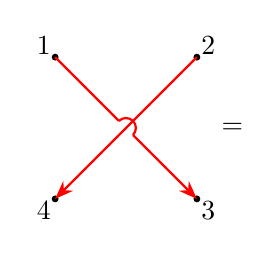
\begin{tikzpicture}[scale=1.8,>=Stealth]
		    
			    \node at (-0.08,-0.08) {$4$};
			    \node at (-0.08,1.08) {$1$};
			    \node at (1.08,1.08) {$2$};
			    \node at (1.08,-0.08) {$3$};
			    \node at (1.25,0.5) {$=$};
			    
			    \draw [fill] (0,0) circle [radius = 0.02];
			    \draw [fill] (1,0) circle [radius = 0.02];
			    \draw [fill] (0,1) circle [radius = 0.02];
			    \draw [fill] (1,1) circle [radius = 0.02];
			    
			    \draw (1,0) [<-,thick,red] -- (0.55,0.45);
			    \draw [thick, red] (0.45,0.55) arc (135:-45:0.07);
			    \draw [thick, red] (0.45,0.55) -- (0,1);
			    \draw [->,thick,red](1,1) -- (0,0);
	
		    \end{tikzpicture}
		    \begin{tikzpicture}[scale=1.8,>=Stealth]
		    
			    \node at (-0.08,-0.08) {$4$};
			    \node at (-0.08,1.08) {$1$};
			    \node at (1.08,1.08) {$2$};
			    \node at (1.08,-0.08) {$3$};
			    \node at (1.25,0.5) {$+$};
			    
			    \draw [fill] (0,0) circle [radius = 0.02];
			    \draw [fill] (1,0) circle [radius = 0.02];
			    \draw [fill] (0,1) circle [radius = 0.02];
			    \draw [fill] (1,1) circle [radius = 0.02];
			    
			    \draw [<-,thick,red](1,0) -- (1,1);
			    \draw [->,thick,red](0,1) -- (0,0);
	
		    \end{tikzpicture}
		    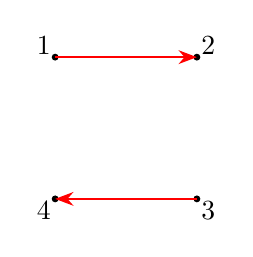
\begin{tikzpicture}[scale=1.8,>=Stealth]
		    
			    \node at (-0.08,-0.08) {$4$};
			    \node at (-0.08,1.08) {$1$};
			    \node at (1.08,1.08) {$2$};
			    \node at (1.08,-0.08) {$3$};
			    
			    \draw [fill] (0,0) circle [radius = 0.02];
			    \draw [fill] (1,0) circle [radius = 0.02];
			    \draw [fill] (0,1) circle [radius = 0.02];
			    \draw [fill] (1,1) circle [radius = 0.02];
			    
			    \draw [->,thick,red](0,1) -- (1,1);
			    \draw [->,thick,red](1,0) -- (0,0);
	
		    \end{tikzpicture}
		\end{center}
	\caption{Graphical representation of the relation $\textcolor{red}{\agl{1}{3}\agl{2}{4}} = \textcolor{red}{\agl{1}{4}\agl{2}{3}} + \textcolor{red}{\agl{1}{2}\agl{3}{4}}$. Then Schouten identities are equivalent to untying crossings for both the two kinds of edges (red and blue) in the graph.}
    \label{fig:Schouten}
\end{figure}

The planarity of the graph translates into a sharp condition on the adjacency matrices associated to it:
\begin{equation}
	\label{eq:planarity}
	\sum_{l=j+1}^n \sum_{k=i+1}^{j-1} A_{k l} \overset{!}{=} 0 \ \ \ \ \mathrm{if} \ A_{i j} \neq 0\ ,
\end{equation}
for any $i=1,\dots , n$ and $j= i+2,\dots ,n-1$.

This also provides an algorithmic method to write any non-planar structure in terms of planar ones. Indeed, if we consider a graph $(\mathbf{A}_i,\mathbf{S}_i)$ for which, for example, the red edges are non-planar, \textit{i.e.} if in \eqref{eq:planarity} any of the $A_{i,\,k l} \neq 0$, then we can recursively untie the corresponding crossing(s) using
\begin{equation}
	\mathbb{M}(\mathbf{A}_i,\mathbf{S}_i) = \mathbb{M}(\mathbf{A}_i+\mathbf{E}^{(i\,j)}_{(k\,l)},\mathbf{S}_i) + \mathbb{M}(\mathbf{A}_i+\mathbf{F}^{(i\,j)}_{(k\,l)},\mathbf{S}_i)\ ,
\end{equation}
where
\begin{equation}
		E^{(i\,j)}_{(k\,l),\, m n} = 
		\begin{cases}
			- 1 & (m\, n) = (i\, j),\, (m\, n) = (k\, l)\\
			+1 & (m\, n) = (i\, k),\, (m\, n) = (j\, l)\\
			0 & \mathrm{otherwise}
		\end{cases}\, ,
\end{equation}
and
\begin{equation}
		F^{(i\,j)}_{(k\,l),\, m n} = 
		\begin{cases}
			- 1 & (m\, n) = (i\, j),\, (m\, n) = (k\, l)\\
			+1 & (m\, n) = (i\, l),\, (m\, n) = (k\, j)\\
			0 & \mathrm{otherwise}
		\end{cases}\, .
\end{equation}

This algorithm can be used to find a basis of $\mathrm{SU}(2)$ singlets in the tensor product of any finite-dimensional representation of the $\mathrm{SU}(2)$ group. Indeed, any tensor transforming in a representation $\mathbf{2\, q+1}$ can be written as a totally-symmetric tensor $T^{a_1\, \cdots \, a_q} = T^{(a_1\, \cdots \, a_q)}$, where $a_i$ are indices in the fundamental of $\mathrm{SU}(2)$. The singlets are given by contractions of any product of tensors of this kind with $\epsilon_{a_1 a_2} = - \epsilon_{a_2 a_1}$ and the Schouten identities are equivalent to
\begin{equation}
	\epsilon_{[a_1 a_2} \epsilon_{a_3] a_4} = 0\ .
\end{equation}
Then to any tensor $T$ we can associate a vertex with valence $q$, and edges correspond to contractions of two $\mathrm{SU}(2)$ indices through an $\epsilon_{a_i a_j}$. Any loop is then automatically zero because
\begin{equation}
	T^{a_1 \cdots a_i \cdots a_j \cdots a_n} \epsilon_{a_i a_j} = 0\ .
\end{equation}
This observation is useful if we want to apply our methods to select a basis of independent $\mathrm{SU}(2)$ gauge structures (see for example \cite{Huber:2021vnc}) or when we will consider polynomial structures with masses involved, because the little group for massive particles in four dimensions is exactly $\mathrm{SU}(2)$. This could be applied to the Lorentz group $\mathrm{SL}(2,\mathbb{C})$ as well because the finite-dimensional representations are in one-to-one correspondence with the those of $\mathrm{SU}(2)\times \mathrm{SU}(2)$.

\subsubsection{Momentum conservation}

Momentum conservation is more subtle and does not have a clear graph-based interpretation. On the other hand, the classification above allows for a massive simplification and the conditions to be imposed in order to find a basis of spinor structures independent up to both Schouten identities and momentum conservation are very easy.


We can take into account most of the relations coming from momentum conservation just by excluding the momentum of the $n^{\rm th}$-particle from the previous assignment. Then the $n^{\rm th}$-vertex will have valence $(\frac{|h_n|+h_n}{2},\frac{|h_n|-h_n}{2})$\footnote{Fully eliminating the momentum of the $n^{\rm th}$-particle is a matter of choices}. This is equivalent to impose the constraint
\begin{equation}
	p_n = - \sum_{i = 1}^{n-1} p_i\ ,
\end{equation}
and we can \textit{eliminate} from our basis any graph whose adjacency matrices \textit{does not} satisfy the conditions
\begin{equation}
	A_{i n} = 0 \ \ \ \ \mathrm{or}\ \ \ \ S_{i n} = 0\ ,
\end{equation}
for any $i=1,\dots , n-1$.

But this is not the end of the story, because there are $n$ additional momentum conservation conditions which do not involve any insertion of the momentum $n$:
\begin{align}
\label{eq::momcons2}
    0 = 
    \begin{cases}
        \sum\limits_{j=1}^{n-1} \agl{i}{j} \sqr{j}{n} &  h_n>0\\[.5em]
        \sum\limits_{j=1}^{n-1} \agl{n}{j} \sqr{j}{i} &  h_n<0\\
    \end{cases}
\end{align}
which are a consequence of the equation of motion for free particles $p_{n\, \alpha \dot{\alpha}}\, \tlambda_{n}^{\dot{\alpha}}=\, 0 \, = \lambda^{\alpha}_n\, p_{n\, \alpha \dot{\alpha}}$, and
\begin{equation}
\label{eq::momcons1}
	\left(\sum_{i = 1}^{n-1} p_{i \, \alpha \dot{\alpha}}\right)^2 =\sum_{i=1}^{n-2} \sum_{j=i+1}^{n-1} s_{i j} = p_n^2 = 0\ .\\
\end{equation}

As already noticed in the previous section, Schouten identities do not change the valences of vertices in the multigraph, then they do not change the number of momenta associated to each vertex. Then we have to find a set of elements in our planar basis which can be written as a linear combination of the others. Once we have discarded all the polynomial structures in which we find the momentum of the $n^{\rm th}$-particle, we need to carefully discard the structures which \textit{maximise} their appearance in conditions \eqref{eq::momcons2} and \eqref{eq::momcons1}. Since any edge $(1,n)$ or $(n-1,n)$ is planar, the natural choice is to isolate terms where either $p_1$ or $p_{n-1}$ appears\footnote{This is an actual choice between momenta of the $1^{\mathrm{st}}$ and the $n-1^{\mathrm{th}}$ momenta. We could actually choose an equivalent basis by writing \eqref{eq::momcons2} as
\begin{align*}
	&\begin{cases}
		\agl{i}{1} \sqr{1}{n} = - \sum\limits_{j=2}^{n-1} \agl{i}{j} \sqr{j}{n} &  h_n>0\\[1em]
        \agl{n}{1} \sqr{1}{i} = - \sum\limits_{j=2}^{n-1} \agl{n}{j} \sqr{j}{i} &  h_n<0\\
	\end{cases}\ ,\\
	&\begin{cases}
		\agl{1}{n-1} \sqr{n-1}{n} = - \sum\limits_{j=2}^{n-1} \agl{1}{j} \sqr{j}{n} &  h_n>0\\[1em]
        \agl{n}{n-1} \sqr{n-1}{1} = - \sum\limits_{j=2}^{n-1} \agl{n}{j} \sqr{j}{1} &  h_n<0\\
	\end{cases}\ .
\end{align*}
} 
and to write the additional momentum conservation conditions as
\begin{align}
	\label{eq:momconsCond1}
	&\begin{cases}
		\agl{i}{n-1} \sqr{n-1}{n} = - \sum\limits_{j=1}^{n-2} \agl{i}{j} \sqr{j}{n} &  h_n>0\\[1em]
        \agl{n}{n-1} \sqr{n-1}{i} = - \sum\limits_{j=1}^{n-2} \agl{n}{j} \sqr{j}{i} &  h_n<0\\
	\end{cases}\ ,\\
	&\begin{cases}
		\agl{n-1}{1} \sqr{1}{n} = - \sum\limits_{j=2}^{n-2} \agl{n-1}{j} \sqr{j}{n} &  h_n>0\\[1em]
        \agl{n}{1} \sqr{1}{n-1} = - \sum\limits_{j=2}^{n-2} \agl{n}{j} \sqr{j}{n-1} &  h_n<0\\
	\end{cases}\ ,
\end{align}
and
\begin{equation}
	\label{eq:momconsCond2}
	s_{1\, n-1} = - \sum_{j=2}^{n-2} s_{1 j} - \sum_{i=2}^{n-2} \sum_{j=i+1}^{n-1} s_{i j}\ .
\end{equation}
The conditions for the adjacency matrices of the polynomial structures in our basis are trivial. We are going to write them in the case $h_n\leq 0$ for simplicity:
\begin{equation}
	\begin{split}
		A_{n-1\, n} = 0 \ \ \ &\mathrm{or}\  \ \ S_{i\, n-1} = 0\ ,\\
		A_{1\, n} = 0 \ \ \ &\mathrm{or}\ \ \ S_{1\, n-1} = 0\ ,\\
		A_{1\, n-1} = 0 \ \ \ &\mathrm{or}\ \ \ S_{1\, n-1} = 0\ .\\
	\end{split}
\end{equation}
Moreover, equations \eqref{eq:momconsCond1} and \eqref{eq:momconsCond2} provide an algorithmic way of writing linear relations of all the polynomial structures in terms of the elements of our basis.

Checks done in this case:
\begin{itemize}
	\item The procedure seems to rely a lot on the cyclic order chosen for the vertices of the graphs and the momenta which we want to eliminate (using momentum conservation and equation of motion). We checked that the number of elements in the basis does not depend on this choices in many non-trivial examples, involving a large number of particles, also with higher helicity.
	\item We showed that we can find a one-to-one map between graphs and structures, then generating all the graphs we can easily generate all the corresponding structures. We checked numerically that the relations we find through our algorithm are correct.
\end{itemize}

\section{The massive contact-term basis}

The classification of independent structures in massive theories involves more technical considerations, but a generalisation of the method presented above for fully massless theories is possible. The sources of such additional complications are two:
\begin{enumerate}
	\item The little group structures\ ,
	\item The equations of motion involving mass terms\ .
\end{enumerate}
With respect to the massless case, we have additional Schouten identities to take into account for the LG indices.
\begin{itemize}
	\item \textbf{Schouten identities for Lorentz} are taken into account by considering planar graphs. The linear relations are easily found by iteratively untying the crossing. In the massive case, this procedure does not distinguish between massive spinor with contracted and free LG indices.
	\item \textbf{Schouten identities for LG} can involve either a momentum and a spinor with free LG index $p_{i \alpha \dot{\alpha}}\, \widetilde{\lambda}^I_{i \dot{\beta}}$ or $p_{i \alpha \dot{\alpha}}\, \lambda^I_{i \beta}$ or two momenta $p_{i \alpha \dot{\alpha}}\, p_{i \beta \dot{\beta}}$.
	\begin{enumerate}
		\item The latter tells us that we have to associate different vertices in the graph to momenta and free indices spinor (whose LG indices are symmetrised). Schouten identities will be again equivalent to untying crossings:
		\begin{equation}
			p_{i \alpha \dot{\alpha}}\, \widetilde{\lambda}^I_{i \dot{\beta}} = p_{i \alpha \dot{\beta}}\, \widetilde{\lambda}^I_{i \dot{\alpha}} + \epsilon_{\dot{\alpha} \dot{\beta}} p_{i \alpha \dot{\gamma}}\, \widetilde{\lambda}^{I \dot{\gamma}}_{i}
		\end{equation}
		or, equivalently, for the “undotted” spinors.
		\item The former tells us that each momenta must be mapped into an new vertex (with a single red and a single blue edge on the vertex). Again we see that Schouten is equivalent to untying the crossing between lines of the same type:
		\begin{equation}
			p_{i \alpha \dot{\alpha}} p_{i \beta \dot{\beta}} = p_{i \beta \dot{\alpha}} p_{i \alpha \dot{\beta}} + \epsilon_{\alpha \beta} p_{i \alpha \dot{\gamma}} p_{i \beta}^{\dot{\gamma}}
		\end{equation}
		or, equivalently, for the “dotted” indices.
	\end{enumerate}
	Then we find a proliferation of vertices, each particle is associated to a vertex carrying both helicity weight and momenta for massless particles and only spin weight for massive one. For each insertion of massive momenta we need to add a vertex next to the spin vertex of the corresponding particle.
	\item \textbf{Momentum conservation} is now taken identically with respect to the massless case:
	\begin{align}
		p_{n-1} | \mathbf{n} ] &= - \sum_{i=1}^{n-2} p_{i} | \mathbf{n} ] - p_{n} | \mathbf{n} ]\ ,\\
		\langle \mathbf{n}| p_{n-1} & = - \sum_{i=1}^{n-2} \langle \mathbf{n}| p_{i}  - \langle \mathbf{n}| p_{n}\ ,\\
		\langle \mathbf{n}| p_{1} | \mathbf{n-1} ] & = - \sum_{i=2}^{n-2} \langle \mathbf{n}| p_{i} | \mathbf{n-1} ] - \langle \mathbf{n}| p_{n} | \mathbf{n-1} ] - \langle \mathbf{n}| p_{n-1} | \mathbf{n-1} ]\ ,\\
		\langle \mathbf{n-1}| p_{1} | \mathbf{n} ] & = - \sum_{i=2}^{n-2} \langle \mathbf{n-1}| p_{i} | \mathbf{n} ] - \langle \mathbf{n-1}| p_{n} | \mathbf{n} ] - \langle \mathbf{n-1}| p_{n-1} | \mathbf{n} ]\ ,\\
		2\,  p_{1}\cdot p_{n-1} &= m_n^2 - \sum_{i=1}^{n-2} \sum_{j=i+1}^{n-1} 2\, p_{i}\cdot p_{j} - \sum_{i=1}^{n-1} m_i^2\ ,
	\end{align}
	which is not a great manipulation of graphs, but we take systematically.
\end{itemize}
These are the operations on graph to find a basis of contact terms.

The $m_i^2$-terms must be eliminated. From a graphic point of view these terms correspond to two momentum vertices of the same massive particle connected by both the red and the blue edge.

Terms proportional to $p_i |\mathbf{i}] = m_i |\mathbf{i}]$ or $\langle \mathbf{i}| p_i = m_i \langle \mathbf{i}|$ should or should not be eliminated according to the spin of the associate particle. From a graphical point of view, they correspond to a momentum vertex connected to the corresponding spin vertex by an (blue or red) edge.
\begin{itemize}
	\item If $s_i< 1$ then we must eliminate them as they correspond to lower dimension operators multiplied with $m_i$ factor.
	\item If $s_i= 1$ and the spin-vertex is connected to a single momentum vertex by only one edge (either blue or red), then we can keep this term. The reason for this is that we have for any $|\mathbf{i}]\langle \mathbf{i}|$ we have an inverse power of the mass $m_i$ from the polarisation tensor.
	\item If $s_i= 1$ and we have multiple edges of this type, then we eliminate the graph.
\end{itemize}
This method should provide both a contact-term basis and a systematic way of finding all the linear relations between different terms.

\section{The massive minimal amplitudes basis}

% \begin{acknowledgments}
%     SDA is a
% \end{acknowledgments} 
    
\appendix

\section{The spinor helicity formalism: review and conventions}
\label{sec:spinorhelicity}

\section{Rational Kinematics and Massive Momentum Twistors}
    \label{sec:massivetwistors}

\bibliographystyle{JHEP}
\bibliography{papers}

\end{document}

% \documentclass[10pt]{article}

% \usepackage[inner=2cm,outer=2cm,top=2cm,bottom=2cm]{geometry}
% \usepackage[tiny]{titlesec}

% \usepackage{multicol}
% \usepackage{amssymb}

% \begin{document}

% \begin{center}
%     {
%         \Large
%         \textbf{Generic EFT Operator Basis from 4D Spinor Helicity Formalism}
%     } 
% \end{center}

% \begin{center}
%     Stefano De Angelis\\[.35em]
%     \textit{
%         \footnotesize Centre for Theoretical Physics, 
%         School of Physics and Astronomy\\
%         Queen Mary University of London,
%         Mile End Road, London E1 4NS, United Kingdom
%     }
% \end{center}


% \begin{abstract}
%     \noindent hello
% \end{abstract}

% \begin{multicols}{2}
% \section{Introduction}
%     hello
% \end{multicols}

% \end{document}